\section[一维平底势阱中的粒子]{一维平底势阱中的粒子} \label{sec:02.04} % 
% \makebox[5em][s]{} % 短题目拉间距

{\heiti 1.无限深平底势阱}

设势能函数为
\begin{equation}\label{eq24.1}
	V(x)=
	\begin{cases}
		0, &|X|<a \\
		\infty,	&|X|\geqslant a
	\end{cases}
\end{equation}

\begin{wrapfigure}[10]{r}{7em}
	\centering
	\small
	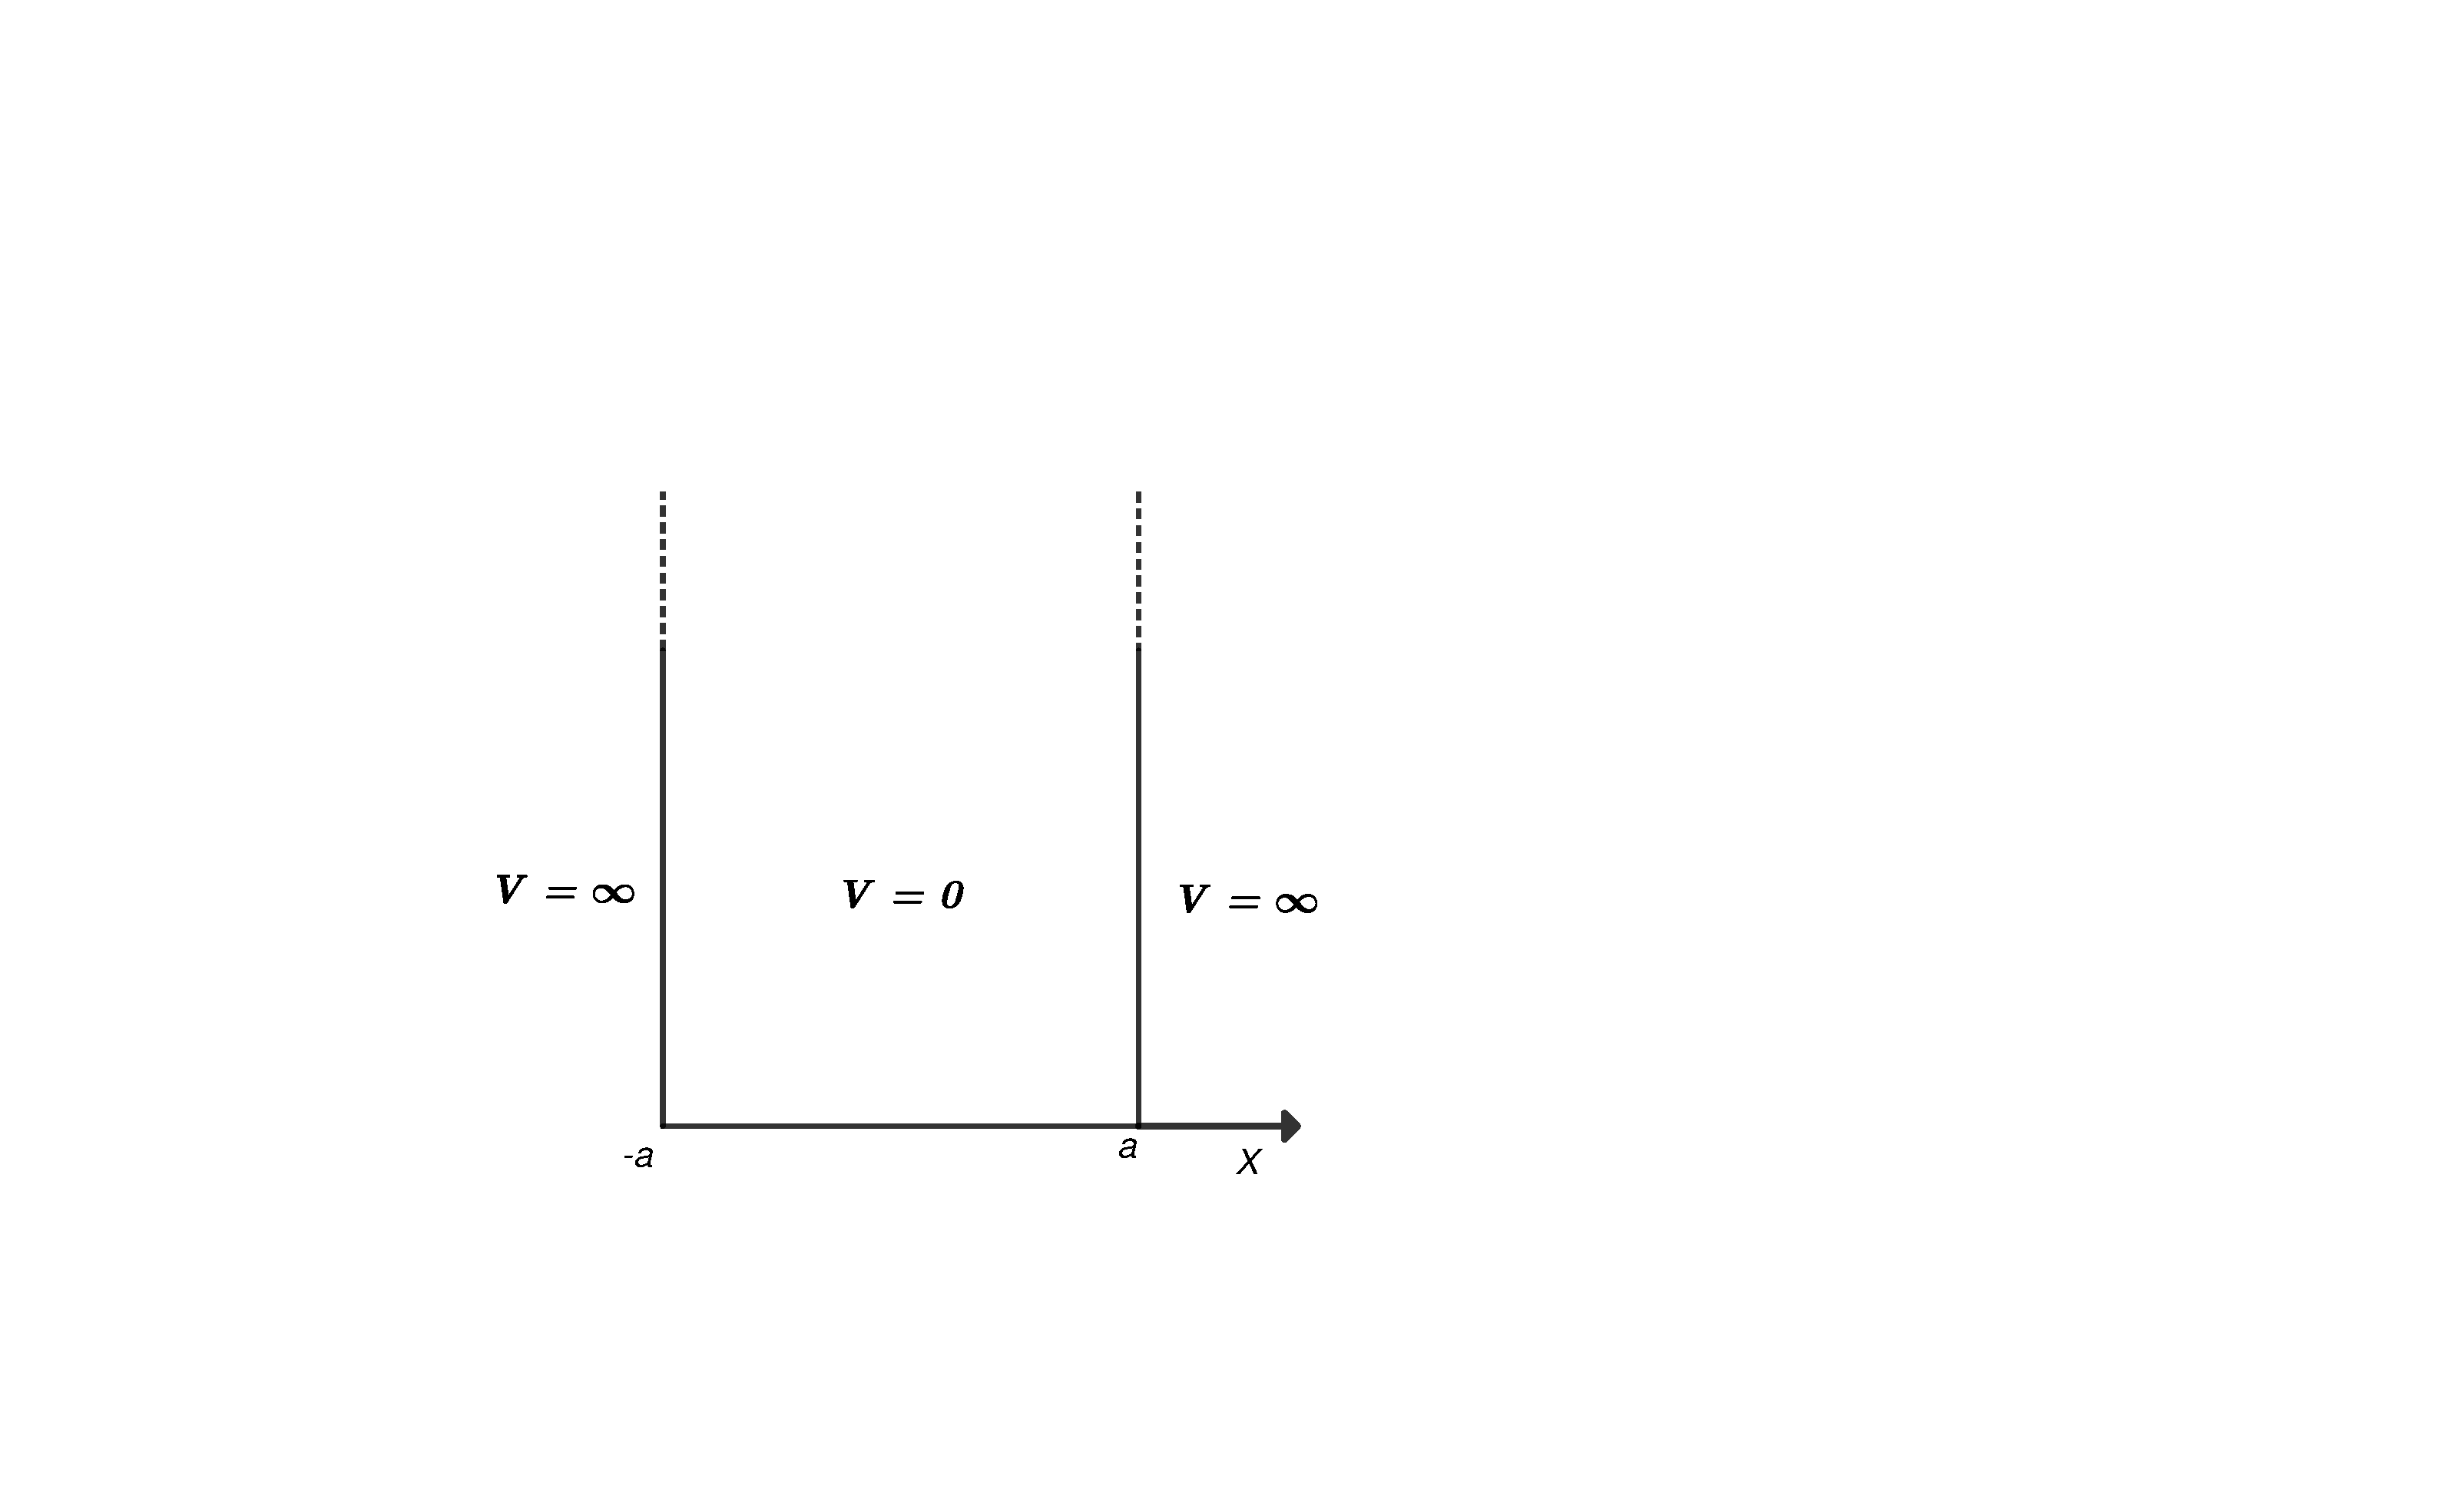
\includegraphics[width=9em]{QM file/figure/2-2}
	\caption{}\label{fig.2-2}
\end{wrapfigure}
如图\ref{fig.2-2}所示.按照$x-V$的图形,这个势场也称为无限深方势阱.粒子在这种势阱中运动时,定态波函数为
\eqlong
\begin{equation}\label{eq24.2}
	\varPsi_{E}(x,t)=\varPsi_{E}(x)e^{-iEt/h}
\end{equation}
$\varPsi_{E}(x)$为空间波函数.由于阱外区域($|x|\geqslant a$)$V=\infty$,$\varPsi$必须等于0,所以可以直接判定
\begin{equation}\label{eq24.3}
	\varPsi_{E}(x)=0,\quad |X|\geqslant a
\end{equation}\eqnormal
阱内$(|x|<a)V=0$,定态薛定谔方程和自由粒子的方程类似,为
\begin{equation}\label{eq24.4}
	\varPsi^{\prime\prime}+k^{2}\varPsi=0,\quad -a<x<a
\end{equation}
其中
\begin{equation}\label{eq24.5}
	k=\frac{\sqrt{2mE}}{\hbar}
\end{equation}
阱内波函数除了满足方程\eqref{eq24.4}外,还要满足边界条件
\begin{equation}\label{eq24.6}
	\varPsi(-a)\approx\varPsi(a)\approx 0
\end{equation}
亦即满足\eqref{eq24.3}式.由于$V(x)$是偶宇称,按照$\S$\ref{sec:02.03}叙述的定理,能量本征态必定有明确的宇称. \eqref{eq24.4}式的特解可以取为$e^{\pm ikx}$或$\cos kx,\sin kx$,前者既不满足边条
件\eqref{eq24.6},也没有宇称性,后二者既有宇称性,也能满足边条件\eqref{eq24.6}.

{\heiti 偶宇称态}

取\eqref{eq24.4}的偶宇称解
\begin{equation*}
	\varPsi(x)=A\cos kx,\quad -a<x<a
\end{equation*}
$A$为归一化系数,边条件\eqref{eq24.6}要求
\begin{equation}\label{eq24.7}
	\cos ka=0,\quad k=\frac{n\pi}{2a},\quad n=1,3,5,\cdots
\end{equation}
因此, 能级为
\begin{equation}\label{eq24.8}
	E_{n}=\frac{\hbar^{2}k^{2}}{2m}=\frac{1}{2m}\bigg(\frac{n\pi\hbar}{2a}\bigg)^{2},\quad
	n=1,3,5,\cdots
\end{equation}
波函数的归一化条件为
\begin{equation}\label{eq24.9}
	\int_{-\infty}^{\infty} |\varPsi|^{2}dx=\int_{-a}^{a} \varPsi^{2}dx=1
\end{equation}
由此定出$A=\frac{1}{\sqrt{a}}$,所以归一化的能量本征函数为
\begin{equation}\label{eq24.10}
	\varPsi_{n}(x)\approx \frac{1}{\sqrt{a}}\cos\frac{n\pi x}{2a},\quad n=1,3,5,\cdots
\end{equation}

{\heiti 奇宇称态}

取\eqref{eq24.4}式的奇宇称解
\begin{equation*}
	\varPsi(x)=A\sin kx,\quad -a<x<a
\end{equation*}
由边条件\eqref{eq24.6}得出
\begin{equation}\label{eq24.11}
	\sin ka=0,\quad k=\frac{n\pi}{2a},\quad n=2,4,6,\cdots
\end{equation}
因此能级为
\begin{equation}\label{eq24.12}
	E_{n}=\frac{1}{2m}\bigg(\frac{n\pi\hbar}{2a} \bigg)^{2},\quad n=2,4,6,\cdots
\end{equation}
归一化的本征函数为
\begin{equation}\label{eq24.13}
	\varPsi_{n}(x)=\frac{1}{\sqrt{a}}\sin\frac{n\pi x}{2a},\quad n=2,4,6,\cdots
\end{equation}
由于粒子被限制在$-a<x<a$范围内运动,只有束缚态,没有游离态,所以全部能级都是量子化的,能级公式为\eqref{eq24.8}、\eqref{eq24.12}式.

$\varPsi_{n}(x)$的图形如图\ref{fig.2-3}所示.在$(-a,a)$间形成驻波,波长为
\begin{equation}\label{eq24.14}
	\lambda=\frac{2\pi}{k}=\frac{4a}{n},\quad n=1,2,3\cdots
\end{equation}
注意$\varPsi_{n}(x)$有$(n + 1)$个波节($\varPsi$的零点).

{\heiti 2.有限深平底势阱}

也称有限深方势阱,势能为
\begin{equation}\label{eq24.14'}
	V(x)=
	\begin{cases} \notag
		-V_{0}, &|X|<a \\
		0,	 &|X|\geqslant a
	\end{cases} \tag{$2.4.14^{\prime}$}
\end{equation}
如图\ref{fig.2-4}所示这种势场可以作为许多实际问题中势场的简单模型,金属中的“自由电子”,原子核中的核子,它们所处的等效势场都可用\eqref{eq24.14}式近似表示,$V_{0}$称为势阱的深度,$2a$是阱的宽度.势能的最小值就是阱内势能$-V_{0}$,由于粒子的定态能量必须大于$V(x)$的平均值,所以$E>-V_{0}$.定态波函数仍可表示成
\begin{equation*}
	\varPsi_{E}(x,t)=\varPsi_{E}(x)e^{-iEt/h}
\end{equation*}
在阱内和阱外,定态薛定谔方程具有不同的构造.
\begin{figure}
	\centering
	\begin{minipage}[h!]{12em}
		\centering
		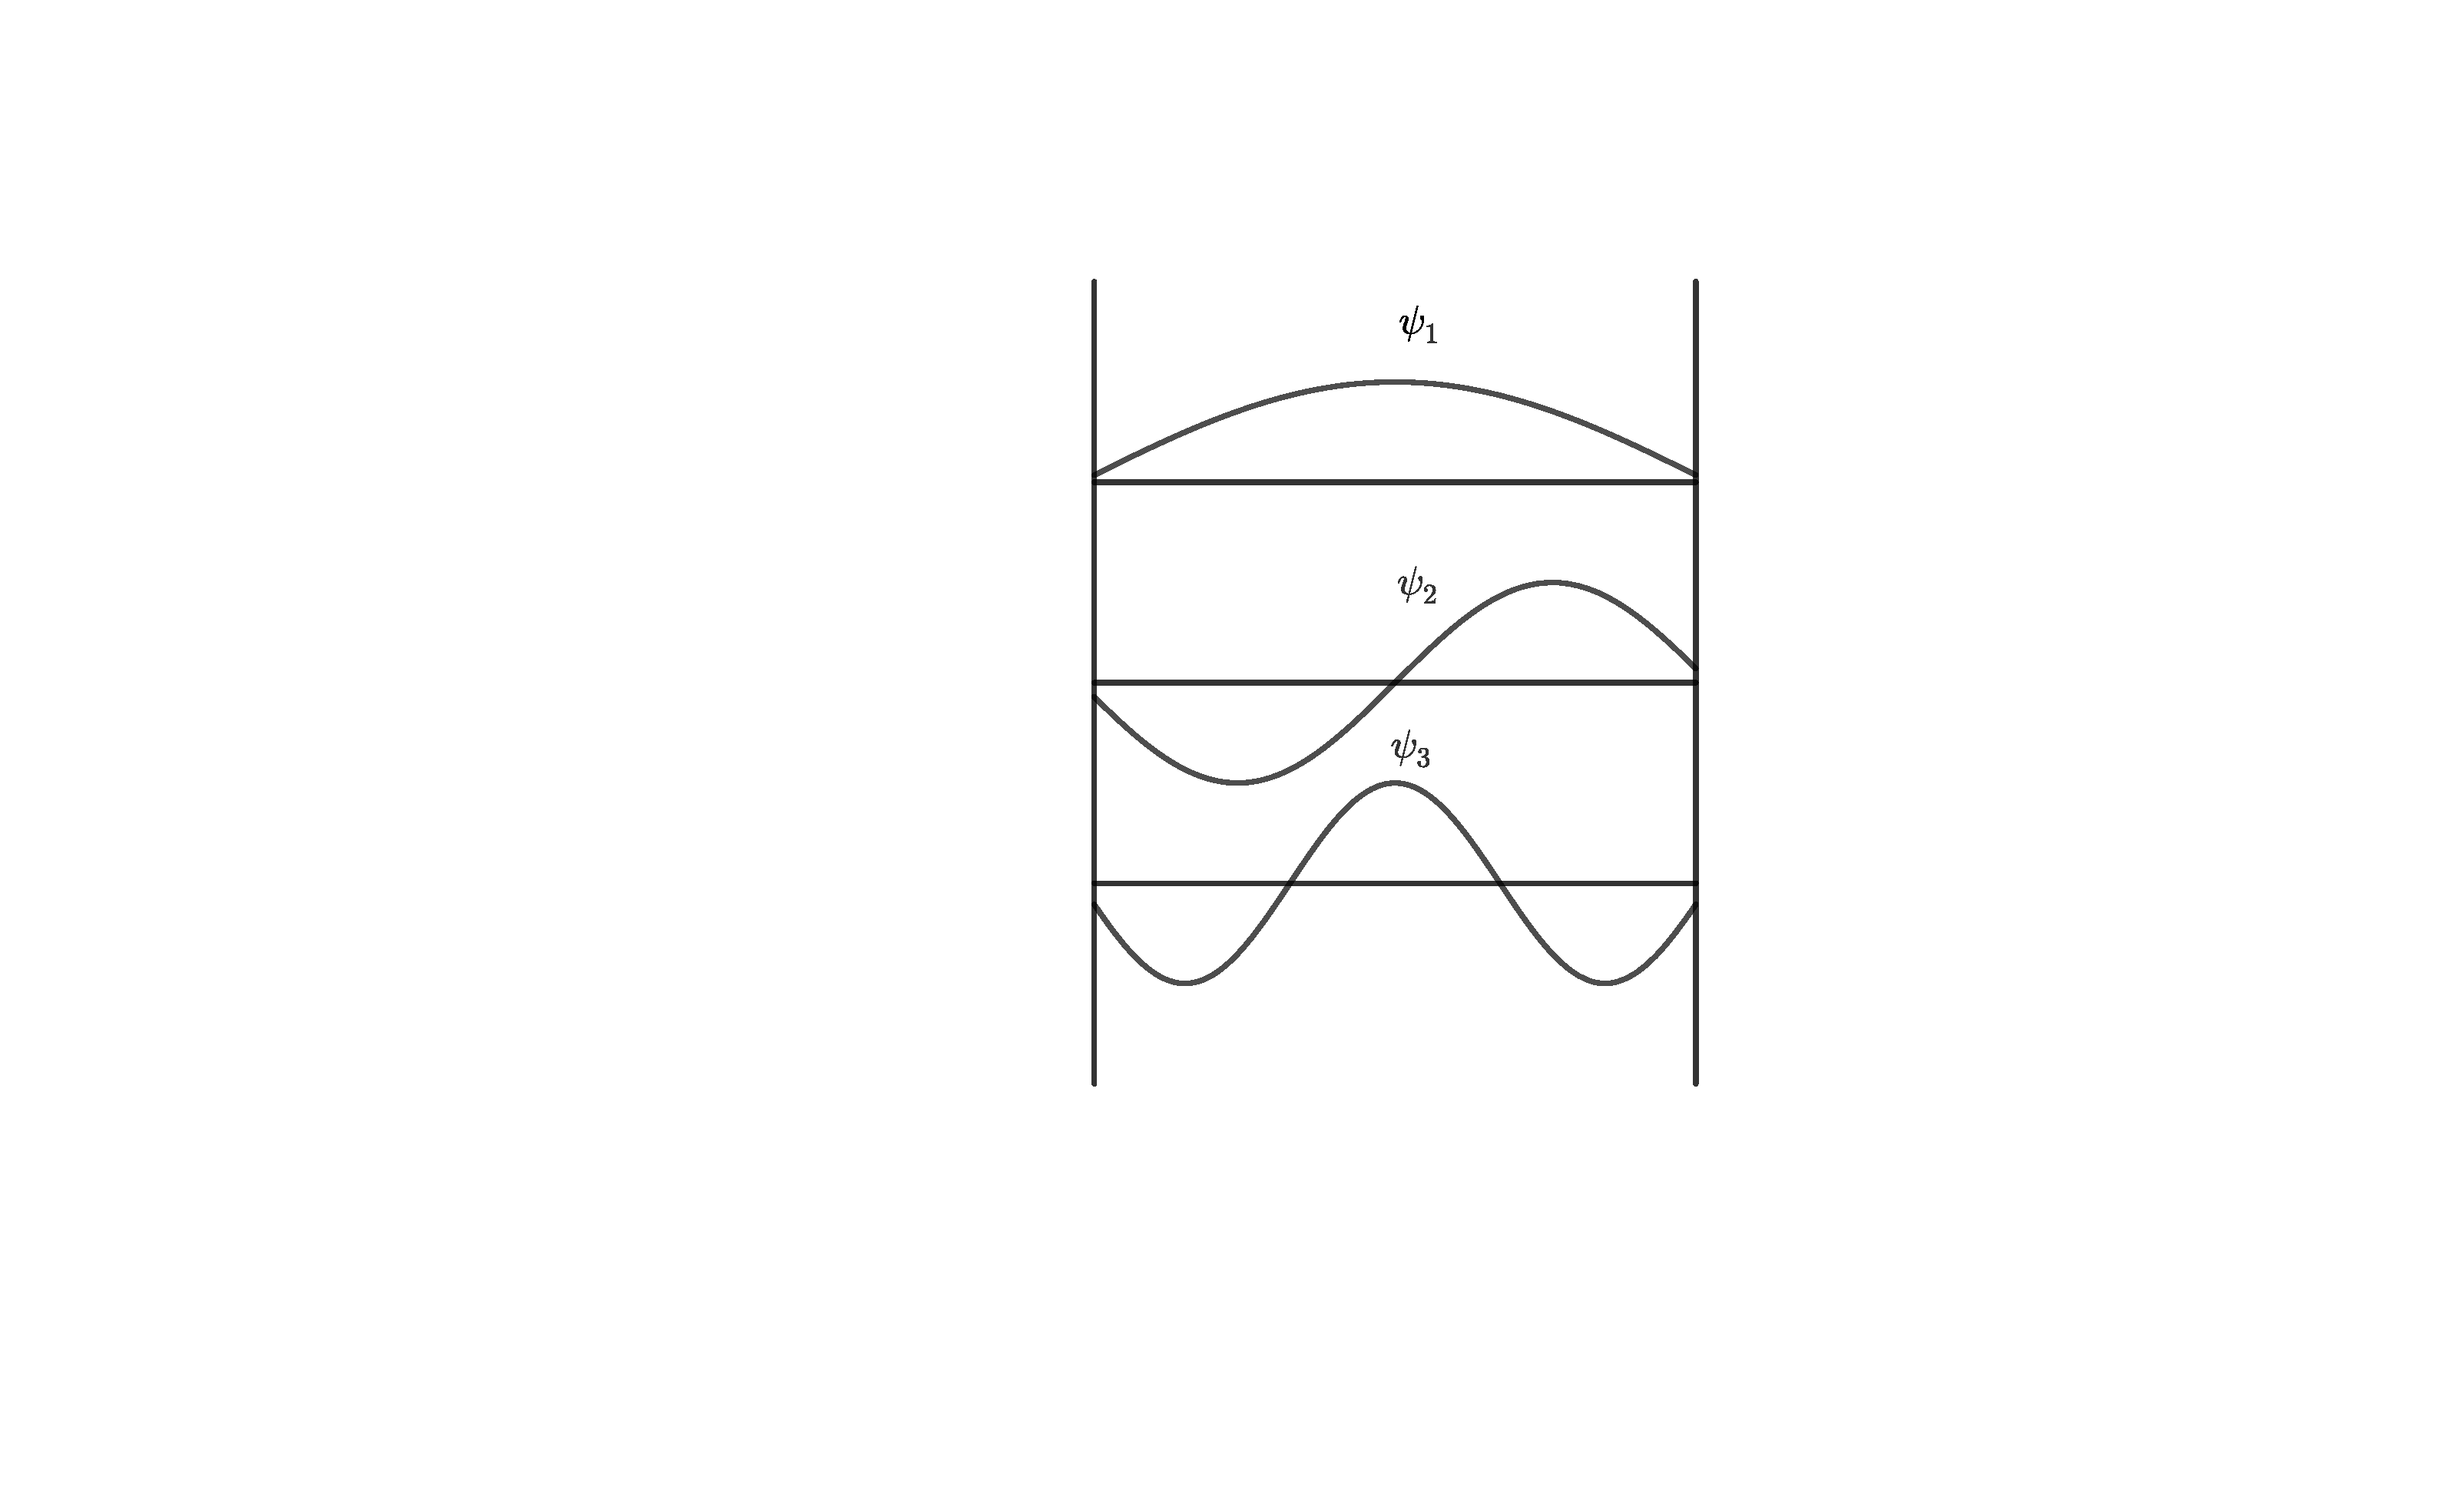
\includegraphics[width=9em]{QM file/figure/2-3}
		\caption{}\label{fig.2-3}
	\end{minipage}
	\begin{minipage}[h!]{12em}
		\centering
		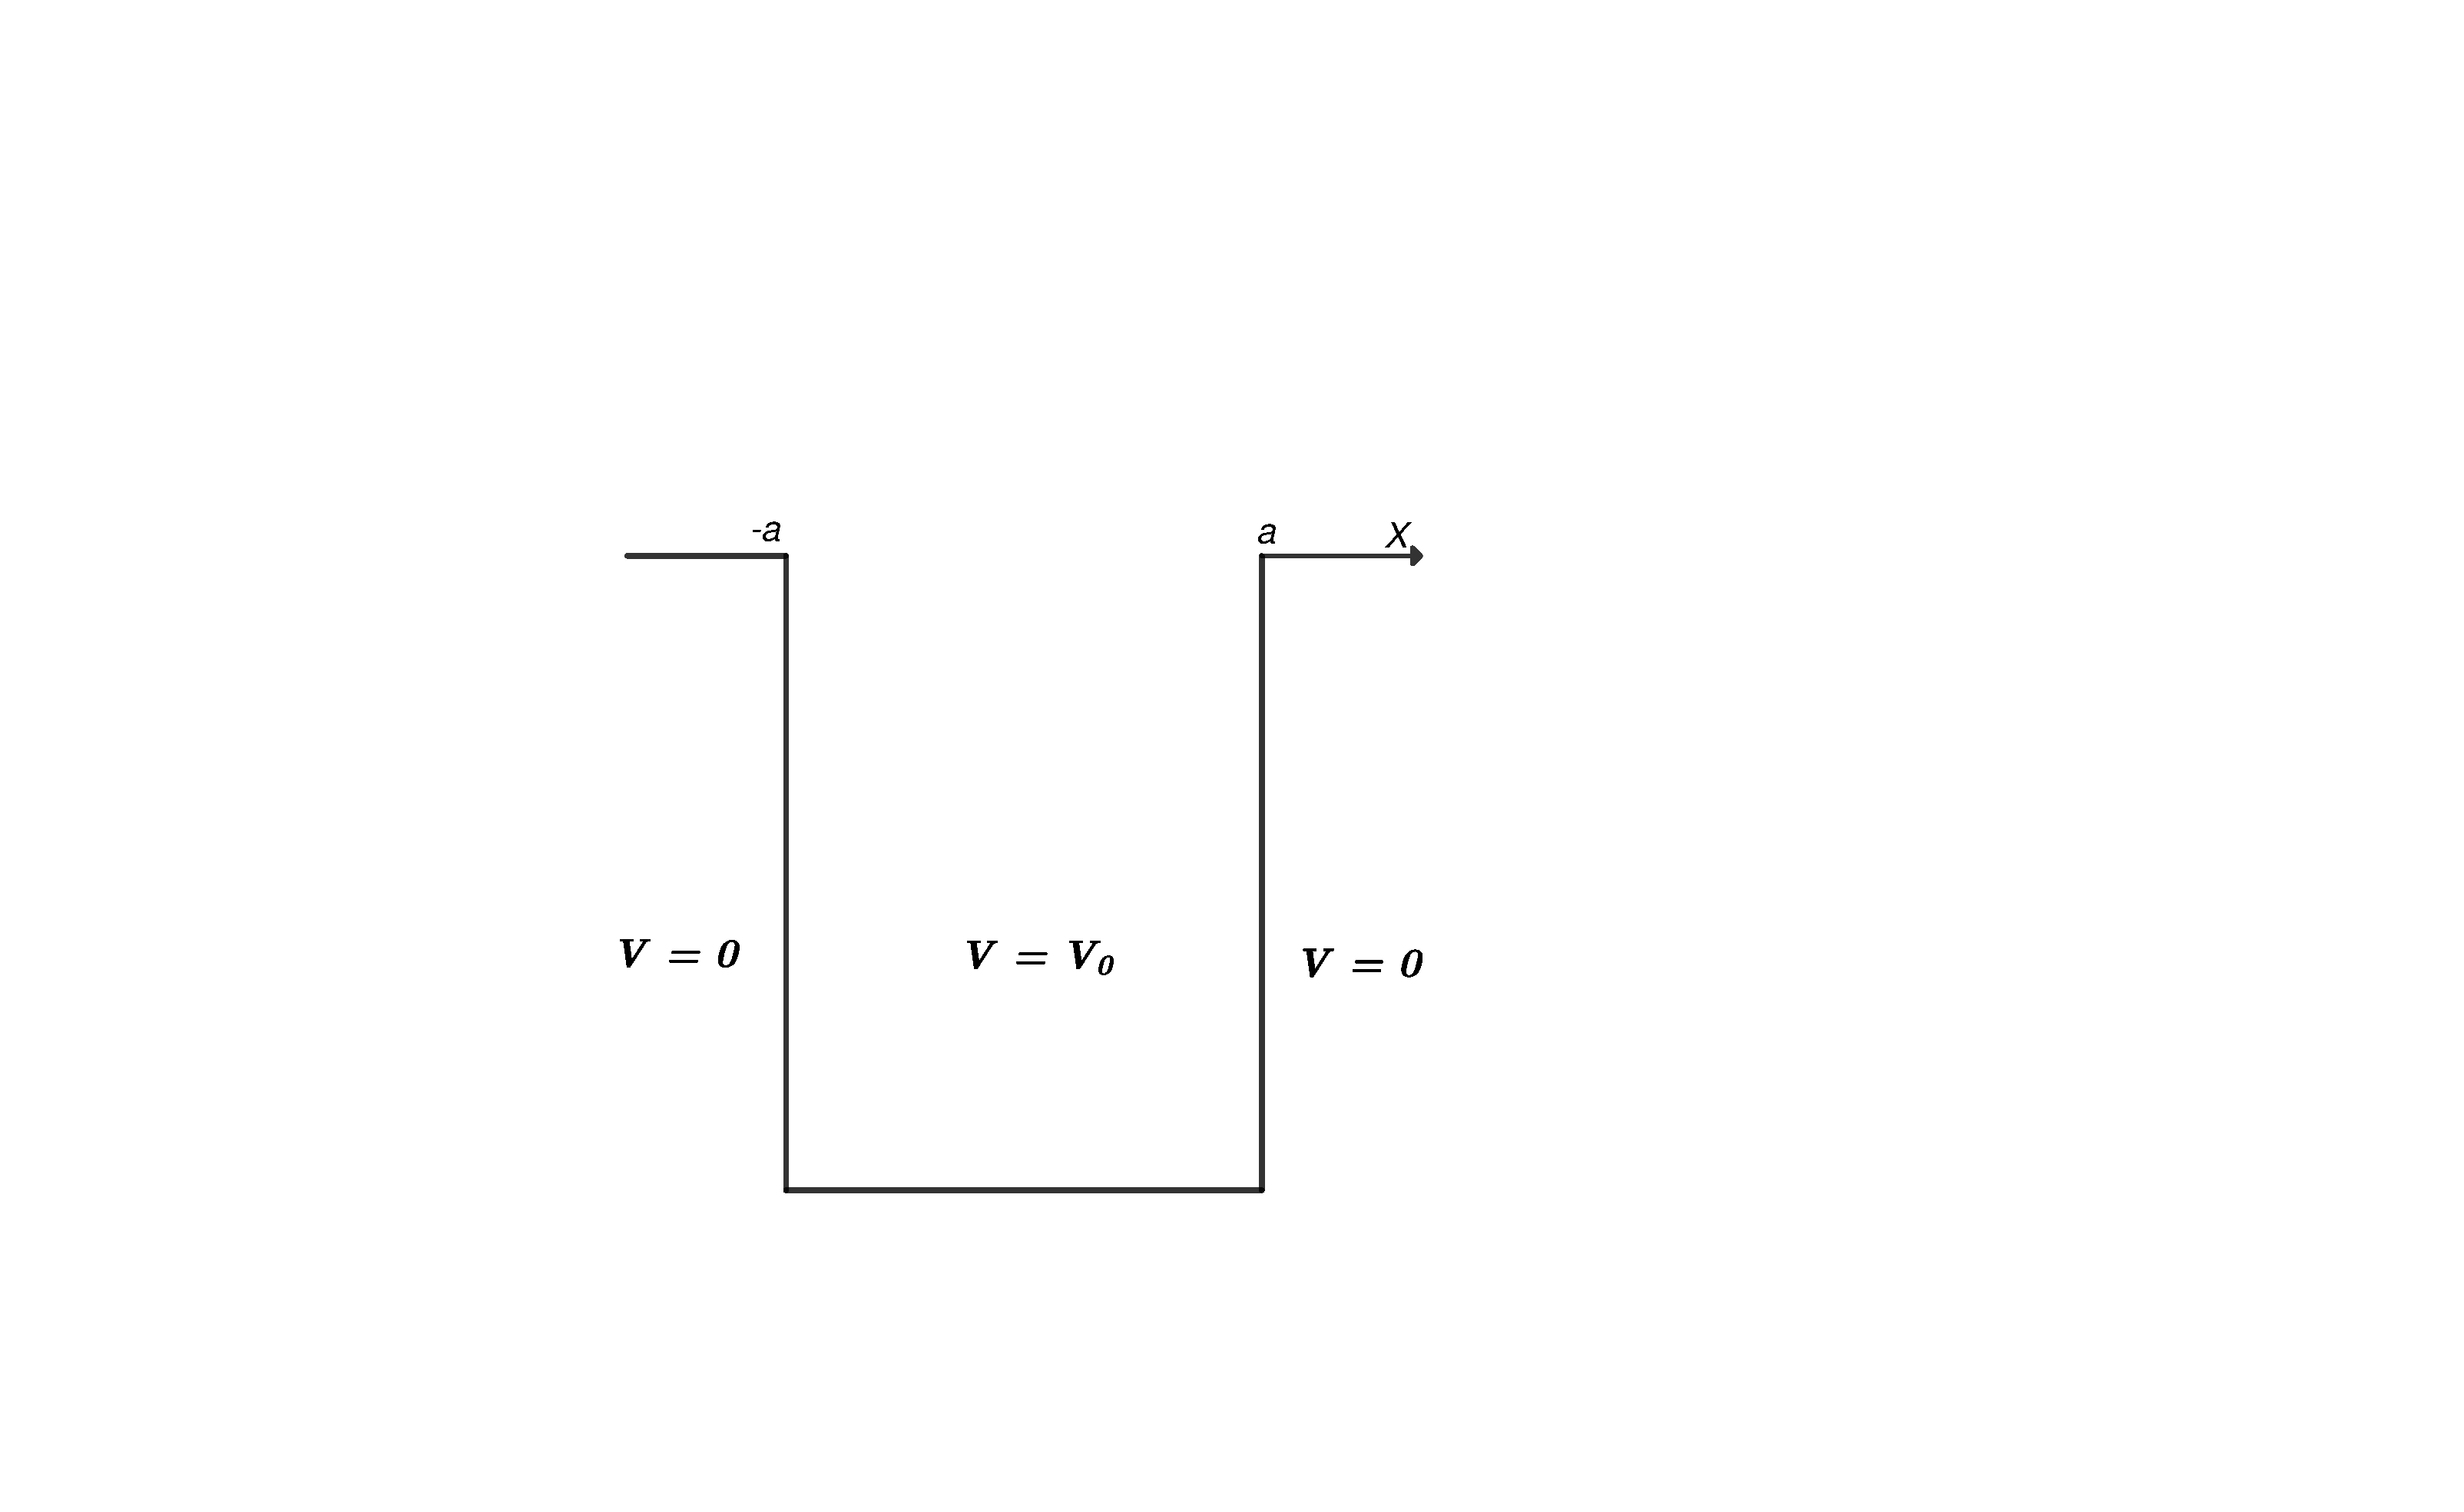
\includegraphics[width=9em]{QM file/figure/2-4}
		\caption{}\label{fig.2-4}
	\end{minipage}
\end{figure}

阱外$(|x|\geqslant a)$.$V(x)=0$ ,定态薛定谔方程为
\begin{equation}\label{eq24.15}
	\varPsi^{\prime\prime}+\frac{2mE}{\hbar^{2}}\varPsi=0,\quad |x|\geqslant a
\end{equation}

阱内$|x|<a$.$V(x)=-V_{0}$,定态薛定谔方程为
\begin{equation}\label{eq24.16}
	\varPsi^{\prime\prime}+\frac{2mE}{\hbar^{2}}(E+V_{0})=0,\quad |x|\geqslant a
\end{equation}
由于$E>-V_{0},E+V_{0}>0$,令
\begin{equation}\label{eq24.17}
	k=\frac{\sqrt{2}m(E+V_{0})}{\hbar}
\end{equation}
则\eqref{eq24.16}式可以写成
\begin{equation*}\label{eq24.16'}
	\varPsi^{\prime\prime}+k^{2}\varPsi=0	\tag{$2.4.16^{\prime}$}
\end{equation*}
和无限深势阱的\eqref{eq24.4}式相似($k$的定义不同).\eqref{eq24.16'}式的两个基本解可以取为$\cos kx$和$\sin kx$元,前者为偶宇称,后者为奇宇称.

对于\eqref{eq24.15}式,$E>0$和$-V_{0}<E<0$有本质区别,前者为游离态,后者为束缚态.我们将着重讨论束缚态.

由于$V(x)$取有限值,$\varPsi(x)$及$\varPsi^{\prime}(x)$是全空间的连续函数,因此由\eqref{eq24.15}式及\eqref{eq24.16'}式分别求出的$\varPsi(x)$及其微商$\varPsi^{\prime}(x)$在$x=\pm a$处应该满足连续条件,以$x=a$处为例, 连续条件为
\setlength{\mathindent}{5em}
\begin{equation*}\label{eq24.17'}
	\varPsi(a-0)=\varPsi(a+0),\quad \varPsi^{\prime}(a-0)=\varPsi^{\prime}(a+0)
	\tag{$2.4.17^{\prime}$}
\end{equation*}\eqnormal
$\varPsi(a\pm 0)$表示,$\varPsi(a\pm\varepsilon),\varepsilon\rightarrow 0$.

{\heiti 束缚态$(-V_{0}<E<0)$}

令
\begin{equation}\label{eq24.18}
	\beta=\frac{\sqrt{-2mE}}{\hbar}>0
\end{equation}
\eqref{eq24.15}式简化成
\begin{equation*}\label{eq24.15'}
	\varPsi^{\prime\prime}\-\beta^{2}\varPsi=0,\quad |x|\geqslant a	\tag{$2.4.15^{\prime}$}
\end{equation*}
两个特解为$e^{\beta x},e^{-\beta x}$.为了保证$\varPsi(x)$有限,必须取
\begin{equation}\label{eq24.19}
	\varPsi(x)=
	\begin{cases}
		Ce^{-\beta x},  & x\geqslant a 		\\
		C^{\prime}e^{\beta x},	& x\leqslant -a
	\end{cases}
\end{equation}
即阱外波函数为指数衰减型这样,当$x\rightarrow\pm\infty$,$\varPsi(x)$迅速趋于0,$ \varPsi(x) $可以满足归一化条件,所以是束缚态.

{\heiti 偶宇称态}$\varPsi(x)\approx\varPsi(-x)$

波函数(不管归一化条件)为
\begin{equation}\label{eq24.20}
	\varPsi(x)=
	\begin{cases}
		Ce^{-\beta x},  & x\geqslant a 		\\
		\cos kx,		& -a<x<a		\\
		Ce^{\beta x},	& x\leqslant -a
	\end{cases}
\end{equation}
利用$ x=a $处$ \varPsi $及$ \varPsi^{\prime} $的连续条件\eqref{eq24.17'},得到
\begin{align}
	C^{-\beta a} &=\cos ka \label{eq24.21} \\
	-\beta Ce^{-\beta a} &=-k\sin ka \label{eq24.22}
	\intertext{二式相除,得到}
	k\tan ka &=\beta	\label{eq24.23}
\end{align}
由于$ K $及$ \beta $均为$ E $的函数,所以\eqref{eq24.23}是$E$所满足的一个超越方程.另外,从$k$和$\beta$的定义式\eqref{eq24.17}、\eqref{eq24.18}还可看出,$k$和$\beta$满足关系
\begin{equation}\label{eq24.24}
	k^{2}+\beta^{2}=\frac{2mV_{0}}{\hbar^{2}}
\end{equation}
\eqref{eq24.23}和\eqref{eq24.24}式就是决定$k$和$\beta$的方程,亦即能级方程,如令
\begin{equation}\label{eq24.25}
	{}
	\begin{cases}
		\xi=ka=\frac{a}{\hbar}\sqrt{2}m(E+V_{0})>0 \\
		\eta=\beta a=\frac{a}{\hbar}\sqrt{-2mE}>0
	\end{cases}
\end{equation}
则能级方程可以写成
\begin{empheq}[left=\empheqlbrace]{align*}
	&\xi\tan\xi=\eta	\tag{$2.4.23^{\prime}$}	\label{eq24.23'}	\\
	&\xi^{2}+\eta^{2}=\frac{2mV_{0}a^{2}}{\hbar^{2}}	\tag{$2.4.24^{\prime}$} \label{eq24.24'}
\end{empheq}
\eqref{eq24.20}式中系数$C$可以由\eqref{eq24.21}式定出,
\begin{equation*}
	C=\cos kae^{\beta_{0}}=\cos\xi\cdot e^{\eta} \tag{$2.4.21^{\prime}$}
\end{equation*}

{\heiti 奇宇称态}$\varPsi(-x)\approx-\varPsi(x)$

波函数为
\begin{equation}\label{eq24.26}
	\varPsi(x)=
	\begin{dcases}
		C^{\prime}e^{-\beta x},  & x\geqslant a 		\\
		\sin kx,		& -a<x<a		\\
		-C^{\prime}e^{\beta x},	& x\leqslant -a
	\end{dcases}
\end{equation}
类似的步骤求得
\setlength{\mathindent}{12em}
\begin{align}
	& \xi\cos\xi=-\eta \label{eq24.27}	\\
	& C^{\prime}=\sin\xi\cdot e^{\eta}	\label{eq24.28}
\end{align}
\eqnormal
\eqref{eq24.27}式和\eqref{eq24.24'}式一起构成能级方程.

{\heiti 能谱}

能级方程\eqref{eq24.23'},\eqref{eq24.24'}.\eqref{eq24.27}可以用数值解法或图解法处理.下面介绍图解法.在$\xi-\eta$图上将\eqref{eq24.23'}、\eqref{eq24.27}式和\eqref{eq24.24'}式分别画成曲线,它们的交点所对应的$\eta$值就代表[通过\eqref{eq24.25}式]能量特征值.
\begin{figure}[!h]
	\centering
	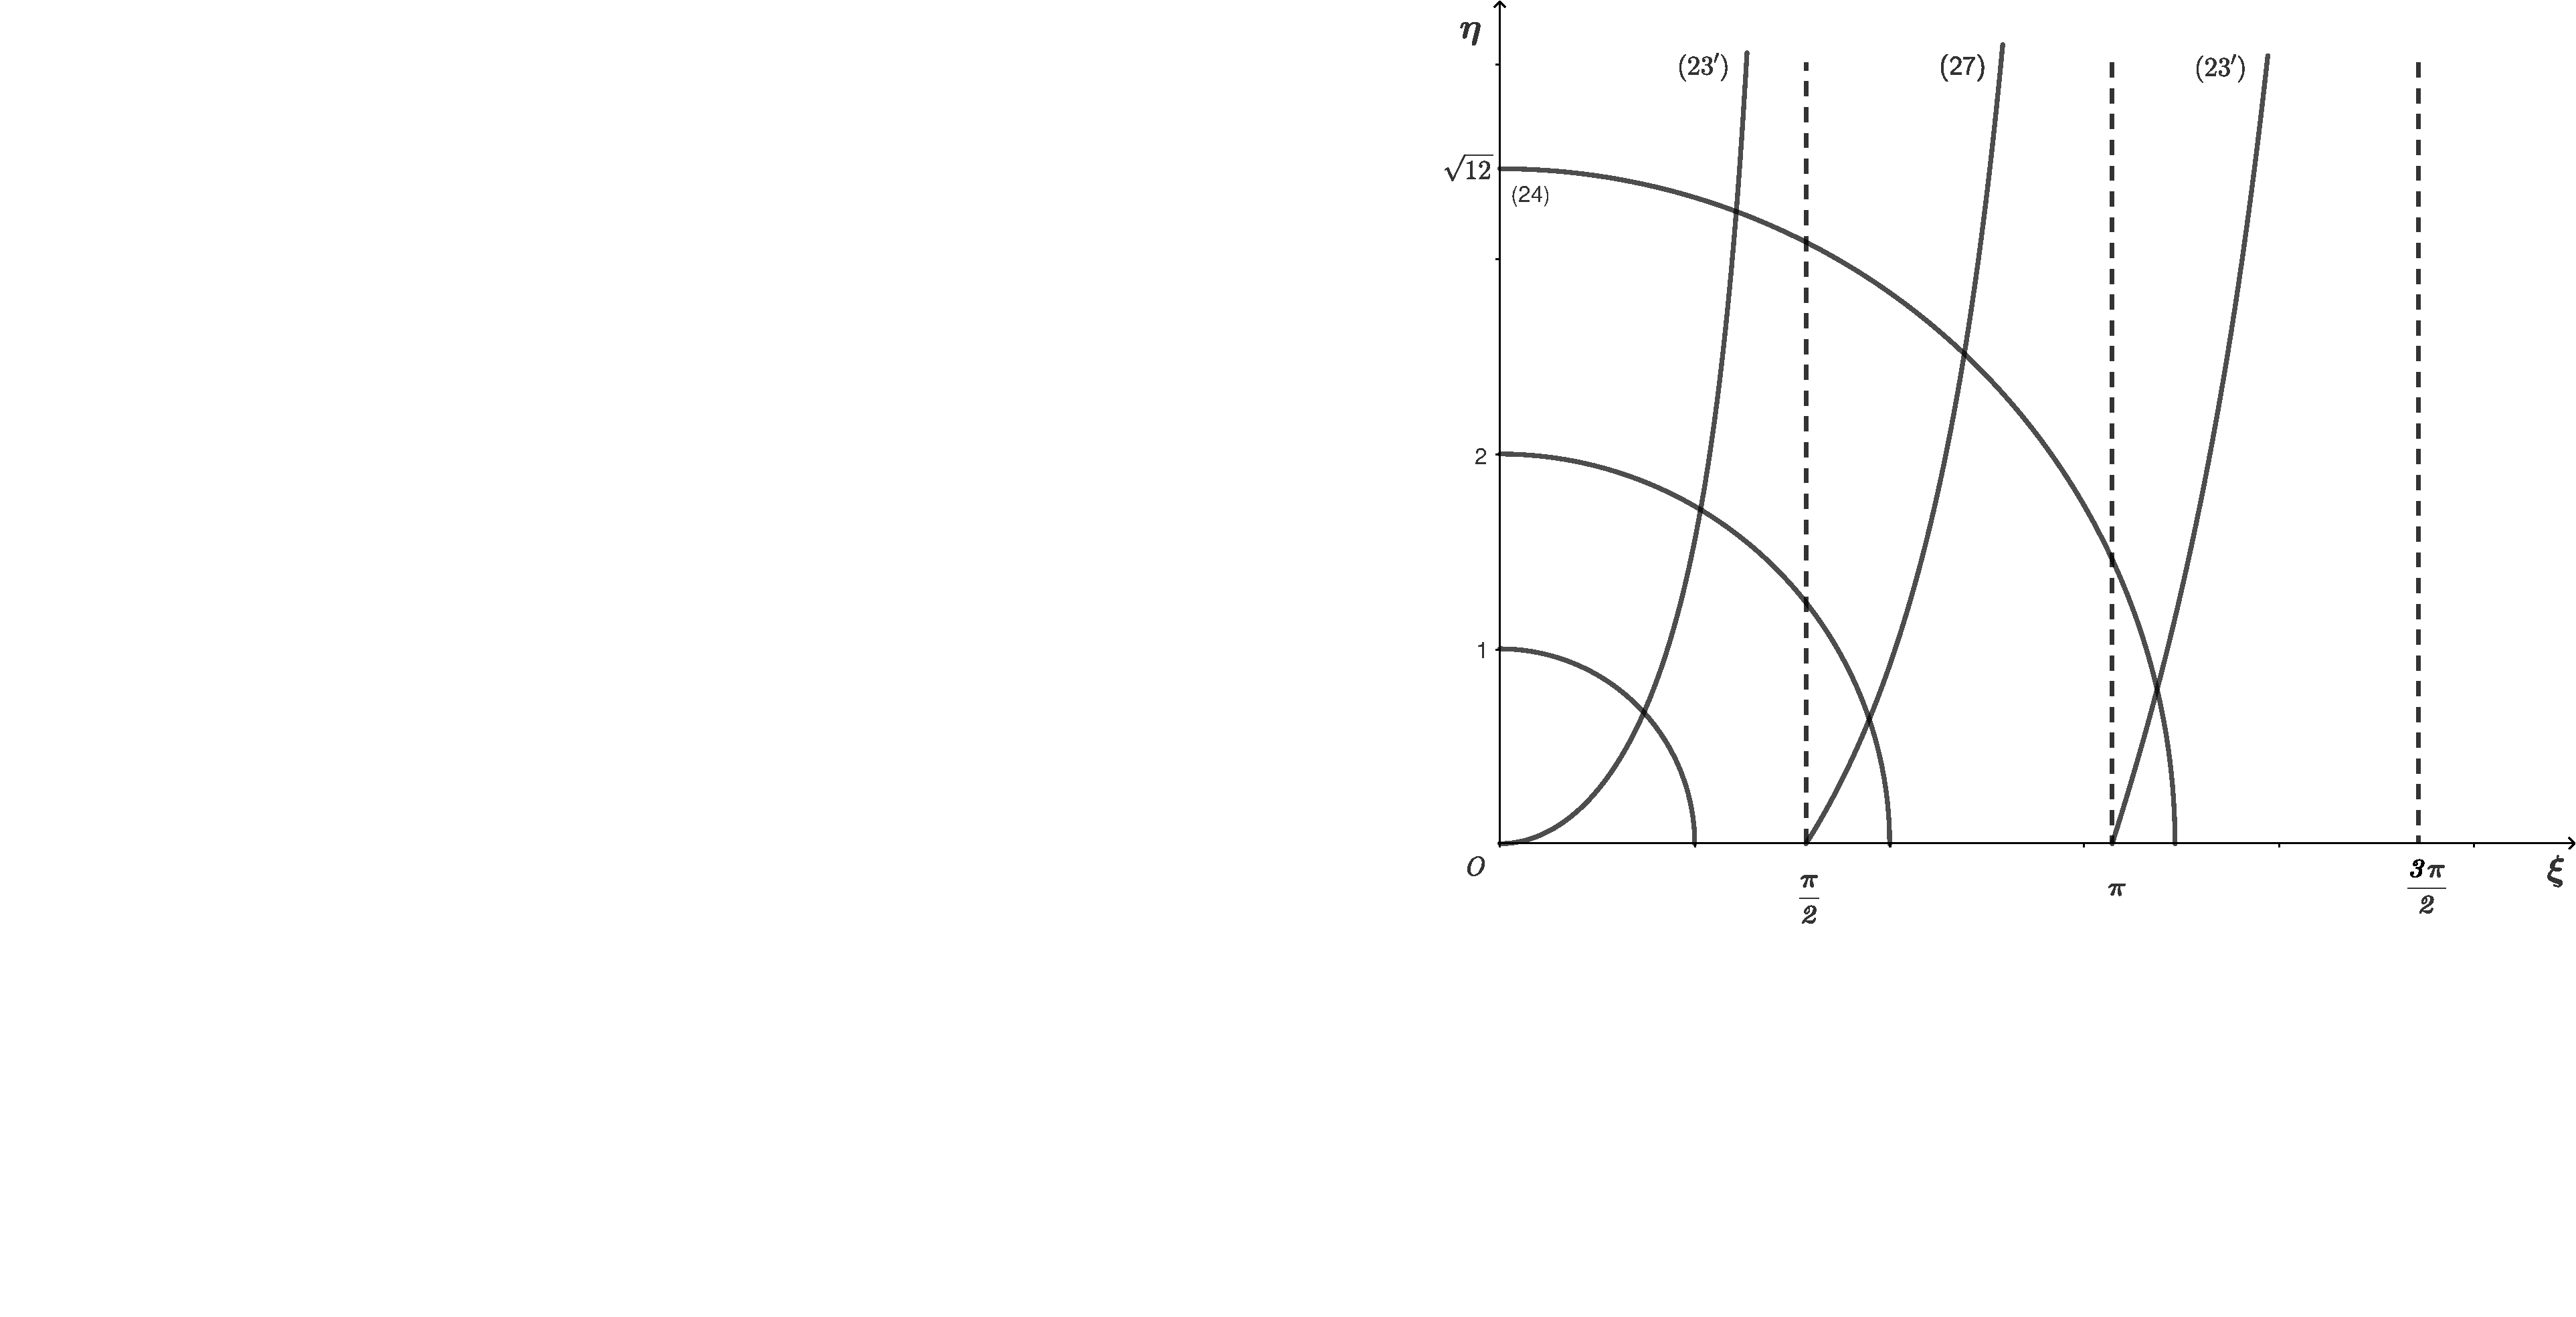
\includegraphics[width=4cm,clip]{QM file/figure/2-5}
	\caption{}\label{fig.2-5}
\end{figure}
束缚态能谱完全取决于$\dfrac{2mV_{0}a}{\hbar}$的数值.图\ref{fig.2-5}就$\dfrac{2mV_{0}a}{\hbar}$的三种特殊值给出了$(\xi,\eta)$值的图解.精确的数值可由数值解法求出,如表\ref{lab.2-1}所示.
\begin{table}[!h]
	\begin{center}
		\caption{}\label{lab.2-1}
		\begin{tabular}{c|c|c|c|c|c}
			\hline 
			\multirow{2}{*}{$\dfrac{2mV_{0}a}{\hbar}$} & \multirow{2}{*}{$\xi$} & \multirow{2}{*}{$\eta$} & \multirow{2}{*}{宇称} & \multirow{2}{*}{$E_{n}$(能级编号)} & \multirow{2}{*}{$\dfrac{4\xi^{2}}{n^{2}\pi^{2}}$} \\ 
			&  &  &  &  &  \\ \hline
			1 & 0.7391 & 0.6736 & 偶 & $E_{1}$ & 0.2214 \\ \hline
			\multirow{2}{*}{4} & 1.0299 & 1.7145 & 偶 & $E_{1}$ & 0.4299 \\ \cline{2-6}
			& 1.895 & 0.6380 & 奇 & $E_{2}$ & 0.3640 \\ \hline
			\multirow{3}{*}{12} & 1.2130 & 3.2448 & 偶 & $E_{1}$ & 0.5964 \\ \cline{2-6}
			& 2.3830 & 2.5142 & 奇 & $E_{2}$ & 0.5754 \\ \cline{2-6}
			& 3.3723 & 0.7922 & 偶 & $E_{3}$ & 0.5121 \\ \hline
			\multirow{2}{*}{$\bigg(\dfrac{10\pi}{2}\bigg)^{2}$} & 1.4767 & 15.6384 & 偶 & $E_{1}$ & 0.8837 \\ \cline{2-6}
			& 2.9525 & 15.4280 & 奇 & $E_{2}$ & 0.8832 \\ \hline
		\end{tabular}
	\end{center}
\end{table}

由能级方程、图\ref{fig.2-5}和表\ref{lab.2-1}可以看出,有限深平底势阱的能级构造有以下规律:

(1) 偶宇称态至少有一个能级.$\dfrac{2mV_{0}a^{2}}{\hbar^{2}}$,能级总数越多. 相邻的能级,宇称相反. 基态能级为偶宇称.

(2) 从阱底算起的能级高度$(V_{0}+E\propto\xi^{2})$低于无限深势阱的相应能级高度.\ref{lab.2-1}最后一列是两种势阱能级高度的比值.当$\dfrac{2mV_{0}a^{2}}{\hbar^{2}}$逐渐增大时,能级总数越来越多,最低的那些能级$\bigg(n\leqslant\dfrac{2a\sqrt{2mV_{0}}}{\pi\hbar}\bigg)$高度逐渐接近无限深势阱的能级高度.

(3) 从阱口算起的能级深度$(-E\propto\eta^{2})$随$\dfrac{2mV_{0}a^{2}}{\hbar^{2}}$增加而增加.每当$\dfrac{2mV_{0}a^{2}}{\hbar^{2}}$超过$\bigg(\dfrac{n\pi}{2}\bigg)^{2}$,阱口即出现一个新能级$(E_{n+1}\sim 0^{-})$能级总数等于
\begin{empheq}{equation}\label{eq24.29}
	n_{max}=1+\big[\frac{2a\sqrt{2mV_{0}}}{\pi\hbar}\big]
\end{empheq}
$[x]$表示不大于$x$的最大整数.

{\heiti 3. $\delta$势阱}

对于有限深方势阱\eqref{eq24.14}式,显然
\begin{empheq}{equation}\label{eq24.30}
	\int_{-\infty}^{\infty}V(x)dx=-2V_{0}a \overset{\text{定义}}{=} -\gamma
\end{empheq}
如果$V_{0}\rightarrow\infty,a\rightarrow 0$,同时保持$\gamma=2V_{0}$.$a$为有限值,就得到一个无限深而又无限窄并满足\eqref{eq24.30}式的势阱,称为$\delta$势阱,其$V(x)$可以写成
\begin{empheq}{equation}\label{eq24.31}
	V(x)=-\gamma\delta(x),\quad\gamma>0
\end{empheq}
由于仅当$ x=0 $,$\delta(x)$才不为0,而且
\begin{empheq}{equation}\label{eq24.32}
	\int_{-\infty}^{\infty}\delta(x)dx=1
\end{empheq}
所以由\eqref{eq24.31}式定义的$ V(x) $显然满足\eqref{eq24.30}式.

在$\delta$势阱中运动的粒子,参量$\frac{2mV_{0}a^{2}}{\hbar^{2}}\rightarrow 0$,所以只有一个束缚态$(E<0)$,波函数为偶宇称,满足定态薛定谔方程
\begin{empheq}{equation}\label{eq24.33}
	\varPsi^{\prime\prime}+\frac{2m\gamma}{\hbar^{2}}\delta(x)\varPsi+\frac{2mE}{\hbar^{2}}\varPsi=0
\end{empheq}
对上式积分,$\int_{-\varepsilon}^{\varepsilon}\cdots dx$,并令$\varepsilon\rightarrow 0$,得到
\setlength{\mathindent}{4em}
\begin{empheq}{equation}\label{eq24.34}
	\varPsi^{\prime}(0^{+})-\varPsi(0^{-})=-\frac{2m\gamma}{\hbar^{2}}\int_{-\varepsilon}^{\varepsilon}\delta(x)\varPsi(x)dx=-\frac{2m\gamma}{\hbar^{2}}\varPsi(0)
\end{empheq}
\eqnormal
$\varPsi^{\prime}$即$\varPsi^{\prime}(\pm\varepsilon)$,$\varepsilon\rightarrow 0$.由上式可见,如$\varPsi\neq 0$,则在$x=0$处$\varPsi$的左微商和右微商不相等,亦即$x=0$处$\varPsi^{\prime}$产生跃变.在$x\neq 0$处,$\delta(x)=0$,\eqref{eq24.33}式成为
\begin{empheq}{equation}\label{eq24.35}
	\varPsi^{\prime\prime}-\beta^{2}\varPsi=0,\quad \beta=\frac{\sqrt{-2mE}}{\hbar}>0
\end{empheq}
其特解为$e^{\pm\beta x}$,考虑到$x\rightarrow\pm\infty$处,$\varPsi$必须有限,所以
\begin{empheq}{equation*}
	x>0,\varPsi\sim e^{-\beta x};\quad x<0,\varPsi\sim e^{\beta x}
\end{empheq}

{\heiti 偶宇称态}

取\eqref{eq24.35}式的偶宇称解
\begin{align}\label{eq24.36}
	\varPsi(x)=
	\begin{dcases}
		Ae^{-\beta x},	&x>0	\\
		Ae^{-\beta x},	&x<0
	\end{dcases}
\end{align}
其微商为
	\begin{numcases}
		{\varPsi^{\prime}(x)=}
		-A\beta e^{-\beta x},	&\text{$x>0$}	\notag	\\
		A\beta e^{-\beta x},	&\text{$x<0$} \notag
	\end{numcases}
令$x\rightarrow 0$.利用$\varPsi^{\prime}$跃变条件\eqref{eq24.34},容易求出
\begin{equation} \label{eq24.37}
	\beta=\frac{\sqrt{-2mE}}{\hbar}=\frac{m\gamma^{2}}{\hbar^{2}}	
\end{equation}
因此能级为
\begin{equation} \label{eq24.38}
	E=-\frac{\hbar^{2}\beta^{2}}{2m}=-\frac{m\gamma^{2}}{2\hbar}	
\end{equation}
\eqref{eq24.36}式中$A$为归一化常数,利用归一化条件
\begin{empheq}{equation*}
	\int_{-\infty}^{\infty}\varPsi^{2}dx=1
\end{empheq}
容易求出$A=\sqrt{\beta}$,因此归一化的能量本征函数为
\begin{align*}\label{eq24.36'}
	\varPsi(x)=
	\begin{dcases}\notag
		\sqrt{\beta}e^{-\beta x}, &x>0	\\ \tag{$2.4.36^{\prime}$}
		\sqrt{\beta}e^{\beta x}, &x<0
	\end{dcases}
\end{align*}
\begin{wrapfigure}[10]{r}{7em}
	\centering
	\small
	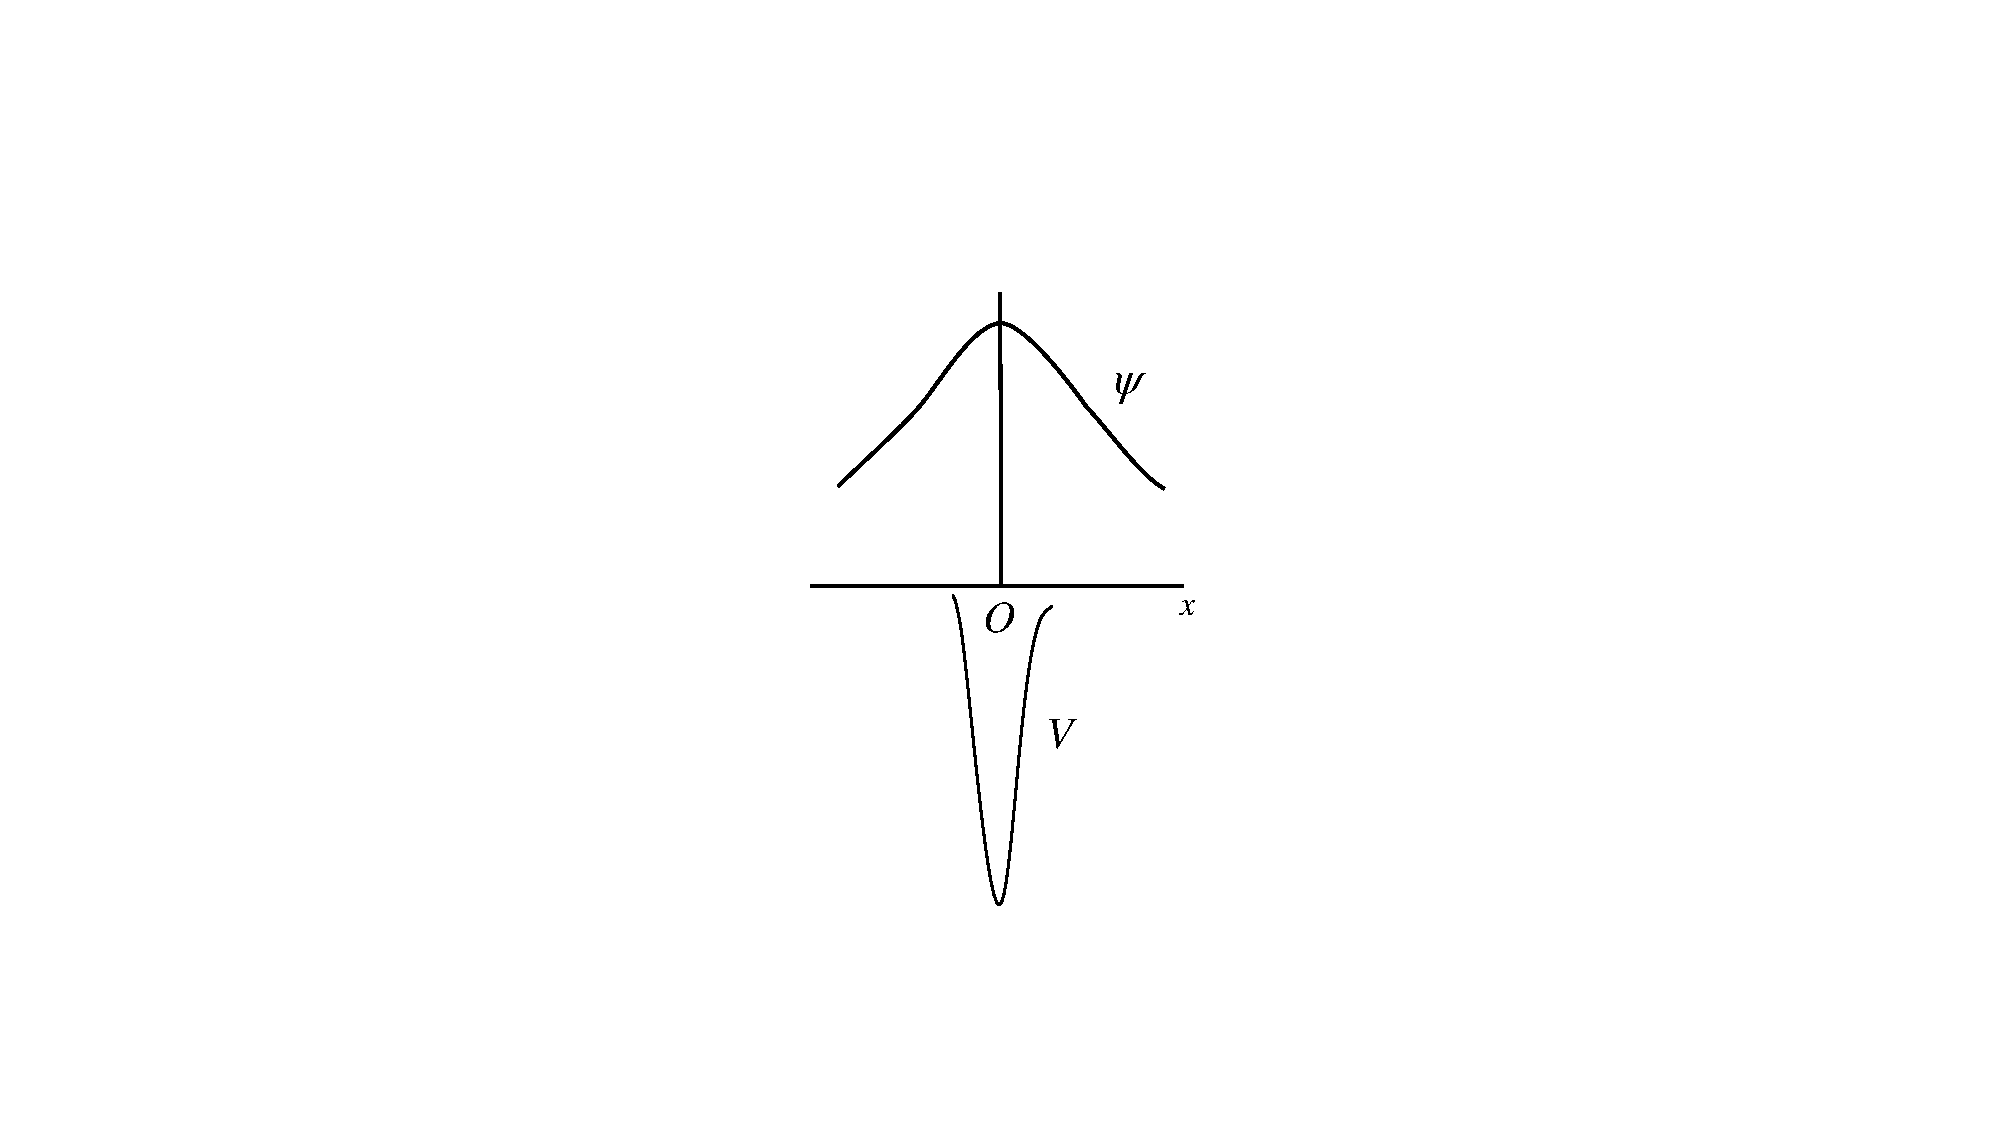
\includegraphics[width=7em,height=9em]{QM file/figure/2-6}
	\caption{}\label{fig.2-6}
\end{wrapfigure}
$\varPsi$的图形如图\ref{fig.2-6}所示,这是$\delta$势阱中的唯一束缚态.

{\heiti 奇宇称态}

\eqref{eq24.35}式的奇宇称解为
\eqlong
\begin{empheq}{equation*}
	{\varPsi(x)=}
	\begin{dcases}
		Be^{-\beta x}	\\
		-Be^{\beta x}
	\end{dcases}
\end{empheq}\eqnormal
满足$\varPsi(-x)=-\varPsi(x)=$.当$x\rightarrow 0,\varPsi(0)=0$,因此$B=0$,即$\varPsi(x)=0$.因此奇宇称束缚态并不存在原因在于:奇宇称态波函数满足$\varPsi(0)=0$,\eqref{eq24.33}式中$\delta(x)$项效果为0,亦即$\delta$势阱对奇宇称态不起作用,粒子运动与自由运动无异,因此$E>0$不存在束缚态.

表征$\delta$势阱性质的特征长度是
\begin{empheq}{equation}\label{eq24.39}
	\frac{1}{\beta}=\frac{\hbar^{2}}{m\gamma}
\end{empheq}
由\eqref{eq24.36'}式容易算出粒子在$|x|<\frac{1}{\beta}$范围内出现概率为
\setlength{\mathindent}{5em}
\begin{empheq}{equation}\label{eq24.40}
	\int_{\frac{1}{\beta}}^{-\frac{1}{\beta}}\varPsi^{2}dx
	=2\beta\int_{0}^{\frac{1}{\beta}}e^{-2\beta x}dx
	=1-e^{-2}=0.8647
\end{empheq}\eqnormal

\example 试利用有限深势阱能级方程导出$\delta$势阱能级公式.

\solution 能级方程为\eqref{eq24.23'}、\eqref{eq24.24'}式, 在条件
\begin{equation*}
	V_{0}\rightarrow\infty,\quad a\rightarrow 0,\quad 2V_{0}a\rightarrow\gamma
\end{equation*}
下,$\frac{2mV_{0}a^{2}}{\hbar^{2}}\rightarrow\frac{2m\gamma^{2}}{\hbar^{2}V_{0}}\rightarrow 0$,由\eqref{eq24.24'}式可知$\xi,\eta$都很小,因此\eqref{eq24.23'}式给出
\begin{equation*}
	\eta=\xi\tan\xi\approx\xi^{2}
\end{equation*}
代入\eqref{eq24.24'}式,得到
\begin{equation*}
	\eta^{2}+\eta-\frac{2mV_{0}a^{2}}{\hbar^{2}}=0
\end{equation*}
解出
\begin{equation*}
	\eta=\frac{1}{2}\bigg(-1+\sqrt{1+\frac{8mV_{0}a^{2}}{\hbar^{2}}} \bigg)
\end{equation*}
由于$ \frac{2mV_{0}a^{2}}{\hbar^{2}} $很小,可取近似
\begin{equation*}
	\sqrt{1+\frac{8mV_{0}a^{2}}{\hbar^{2}}}\approx 1+\frac{4mV_{0}a^{2}}{\hbar^{2}}
\end{equation*}
因此
\begin{equation*}
	\eta=\frac{2mV_{0}a^{2}}{\hbar^{2}}=\beta a,\quad \beta=\frac{2mV_{0}a}{\hbar^{2}}=\frac{m\gamma}{\hbar^{2}}
\end{equation*}
再利用\eqref{eq24.25}式,即得
\begin{equation*}
	E=-\frac{\beta^{2}\hbar^{2}}{2m}=-\frac{2mV_{0}a^{2}}{\hbar^{2}}=-\frac{m\gamma^{2}}{2\hbar^{2}}
\end{equation*}
此即$\delta$势阱能级公式\eqref{eq24.38}.





